\imprimircapa

\imprimirfolhaderosto*

% ---
% Caso a Biblioteca da UDESC forneça, utilize o comando
% ---
% \begin{fichacatalografica}
%     \includepdf{fig_ficha_catalografica.pdf}
% \end{fichacatalografica}

% ---
% Geração da Ficha Catalográfica Via LaTeX
% ---
\begin{fichacatalografica}
  \vspace*{\fill}					% Posição vertical
  \begin{center}					% Minipage Centralizado
    \begin{minipage}[c]{12.5cm}		% Largura

      da Silva, Renan Samuel

      \hspace{0.5cm} \imprimirtitulo  / \imprimirautor. --
      \imprimirlocal, \imprimirdata-

      \hspace{0.5cm} \pageref{LastPage} p. : il. (algumas color.) ; 30 cm.\\

      \hspace{0.5cm} Orientador: \imprimirorientadorRotulo~\imprimirorientador\\

      \hspace{0.5cm}
      \parbox[t]{\textwidth}{Dissertação (mestrado) -- Universidade do Estado de Santa Catarina, Centro de Ciências Tecnológicas, Programa de Pós-Graduação em Computação Aplicada, Joinville, 2019}\\

      \hspace{0.5cm}
      1. Monte Carlo.
      2. Inserção de fragmento.
      3. Problema de Predição de Estrutura de Proteínas.
      4. Controle de Parâmetros.
      5. Clusterização.
      I. Parpinelli, Rafael Stubs.
      II. Universidade do Estado de Santa Catarina.
      III. Centro de Ciências Tecnológicas.
      IV. Programa de Pós-Graduação em Computação Aplicada.

      \hspace{8.75cm} CDU 02:121:005.7\\

    \end{minipage}
  \end{center}
\end{fichacatalografica}

% ---
% Folha de Aprovação
% ---
% Exemplo de folha de aprovação antes da Banca. Após isso, incluia o pdf digitalizado com as assinaturas%
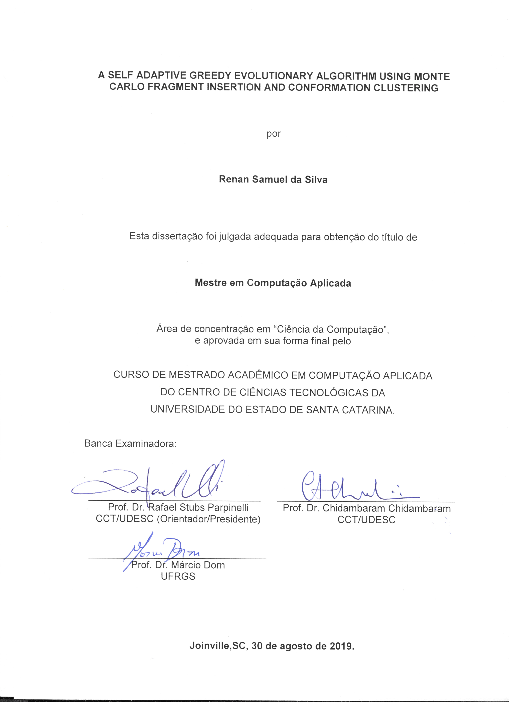
\includepdf{Partes/approval.pdf}
% \begin{folhadeaprovacao}
% 
%   \begin{center}
%     {\ABNTEXchapterfont\bfseries\imprimirautor}
%     \vspace{6em}
% 
%       \ABNTEXchapterfont\bfseries\imprimirtitulo
% 
%   \end{center}
%     \vspace{1em}
%     {\justify
%     This content was submitted to examination board as partial fulfillment to obtain the title of
%       {\ABNTEXchapterfont\bfseries Master in Applied Computing},
%       area of concentration in "Computational Systems", by the Graduate Program in Applied Computing at the College of Technological Science of Santa Catarina State University.}
% 
%       % 		{\justify
%       % 		This Master thesis was considered adequate to obtain the title of
%       %     	{\ABNTEXchapterfont\bfseries Master in Applied Computing},
%       %    		area of concentration in "Computational Systems",
%       %    		and approved in its final form by the Graduate Program in Applied Computing at the College of Technological Science of Santa Catarina State University.}
% 
%   \vspace{3em}
%   \noindent
%   {\bfseries Examination Board:}
%   \assinatura{\textbf{\imprimirorientador} \\ Advisor}
%     \assinatura{\textbf{Dr. Chidambaram Chidambaram} \\ CCT-UDESC}
%     \assinatura{\textbf{Dr. Márcio Dorn} \\ INF-UFRGS}
% 
%     \vspace*{\fill}
%     \begin{center}
%       \imprimirlocal,\,\imprimirfulldata
%     \end{center}
% \end{folhadeaprovacao}

% ---
% Dedicatória
% ---
\begin{dedicatoria}
  To my Father that is no longer with us and to my Mother that always stood by me.
\end{dedicatoria}

% ---
% Agradecimentos
% ---
% TODO: Update agradecimentos
\begin{agradecimentos}
  Firstly I would like to thank my mother, Tatiana. Without her continuous and never ending support
  I would not been here. Not only did she financially and emotionally support me, she also
  did encourage me since I was very young to study and go after my dreams. This shaped me
  into who I am.

  I also would like to deeply thank Rafael Parpinelli for supporting me over this journey
  and helping me push the limits of my knowledge. I also thank all my friends that were with
  me since my first day at the university. In special Andressa Umetsu, Rafael Castro, Vinicius Zuchi,
  Tiago Heinrich,
  Aurelio Grott, Mateus Boiani, William Pereira, Karll Henning, Dalmo Neto, Lucas Zanatta and many others.
  They all made my days more bearable and fun.
  To all the teachers that served both as friends and a role models,
  in special professor Omir. I had the pleasure of working for more than two years with him.
  The experience that I gained while working with him helped define who I am today as an academic.
  To my team leads at JobScore, Thiago and Wesklei,
  who can understand what is like to be working and doing a master
  degree at the same time and helped along the path as well.

  Finally I would like to thank Andressa Umetsu for becoming one of the closest friends that
  I have. Her friendship made me a happier person.
\end{agradecimentos}

% ---
% Epígrafe
% ---
\begin{epigrafe}
  ``It is not because things are difficult that we do not dare, but because we do not dare, things are difficult.''
  \\
  \par
  Seneca, Moral letters to Lucilius/Letter 104, verse 26
\end{epigrafe}

% ---
% RESUMOS
% ---

% ---
% Ao usar o modo twoside (anverso e verso) o resumo não se posiciona na página ímpar.
% Dessa forma, deve-se forçar o resumo para iniciar em uma página ímpar, usando o seguinte comando:
% ---

%\newpage\null\thispagestyle{empty}\newpage

% Inglês
% TODO: Update resumo en
\begin{resumo}
  The Protein Structure Prediction Problem (PSPP) is currently one of the
  most important and challenging open problems in both computer science and
  in structural bioinformatics. Being able to accurately predict protein
  conformations would have a significant impact on several fields.
  Proteinopathies would be better understood, intelligent protein based drugs
  could be designed more easily and the overall understanding of the protein
  functions in organisms would be further increased. Even with the problem being
  several decades old, no viable general solution was found. Currently, only
  small protein are able to be predicted with satisfactory levels of
  accuracy. As such, this work has as its main goal to attempt in improving the
  prediction power of ab initio methods by utilizing an self adaptive
  evolution algorithm using Monte Carlo based fragment insertion and
  conformational clustering. With this, a proven meta heuristic is utilized
  as the core of the conformation sampling process with fragment insertion
  feeding domain specific information into the process. The online parameter
  control allows the method to adapt to proteins of different features
  and also to different stages of the optimization process. The main
  contribution of this work is a novel combination of online parameter
  control, fragment insertion, conformational clustering and metaheuristics.
  In order to assess the performance of the proposed methods they were
  compared against each other and two methods from the literature using
  a series of statistical methods. The proposed methods were then compared
  against several methods in the literature, utilizing only the RMSD. 
  Finally, it was
  concluded that the proposed methods were able to outperform Rosetta, one of
  the state-of-art methods. Furthermore, the RMSD of the protein targets were
  either the best one so far, or the second best in the literature, over more
  than 20 works reviewed.
  \\
  \vspace{\onelineskip}
  \noindent
  \textbf{Keywords}: Monte Carlo, Fragment Insertion, Protein Structure Prediction Problem, Parameter Control, Clustering.
\end{resumo}

% ---
% Ao usar o modo twoside (anverso e verso) o resumo não se posiciona na página ímpar.
% Dessa forma, deve-se forçar o resumo para iniciar em uma página ímpar, usando o seguinte comando:
% ---

%\newpage\null\thispagestyle{empty}\newpage

% Português
% TODO: Update resumo pt-br
\begin{resumo}[Resumo]
  \begin{otherlanguage*}{brazil}
    O Problema de Predição de Estrutura de Proteína é atualmente um dos mais
    importantes e desafiadores problemas em aberto na ciência da computação e
    na bioinformática estrutural. Ser capaz de predizer a estrutura de proteínas
    com acurácia teria um impacto significativo em multiplas áread do
    conhecimento. Proteinopatias seriam melhor entendidas, drogas inteligentes
    baseadas em proteínas poderia ser projetadas mais facilmente e o
    conhecimento em geral de proteínas nos seres vivos seria expandido.
    Apesar do problema de predição ter várias decadas, até hoje nenhuma solução
    generalizada viável foi encontrada. Atualmente, apenas pequenas proteínas
    podem ter sua estrutura predita com um nível desejável de acurária. Deste
    modo, este trabalho tem como principal objetivo tentar melhorar o poder
    preditivo de métodos ab initio através da utilização de um algoritmo
    evolucionário auto adaptativo usando inserçao de fragmentos baseada em
    Monte Carlo e clusterização de conformações. Com isto, uma poderosa meta
    heurística será utilizada como núcleo para o processo de amostragem de
    conformações com a inserção de fragmentos agregando informação do domínio do
    problema. O controle online de parametros permitirá que o método se adapte a
    proteínas de diferentes caracteristicas e também a diferentes etapas do
    processo de otimização. A principal contribuição deste trabalho está na
    inovativa proposta de combinar controle online de parametros, inserção de
    fragmentos, clusterização de conformações e meta heurísticas. Com o objetivo
    de aferir a performance dos métodos propostos, estes foram comparados contra
    dois outros métodos da literatura, utilizando uma série de métodos
    estatísticos. Os métodos propostos foram então comparados contra diversos
    outros na literuatura, utilizando apenas o RMSD. Foi concluído que os
    métodos propostos foram capazes the obter performance superior a Rosetta, um
    os métodos estado da arte. Finalmente, o RMSD das proteínas alvo foram ou
    a melhor ou a segunda melhor encontradas na literatura, dentre mais de 20
    trabalhos analisados.
    \\
    \vspace{\onelineskip}
    \noindent
    \textbf{Palavras-chave}: Monte Carlo, Inserção de fragmento, Problema de Predição de Estrutura de Proteínas, Controle de Parâmetros, Clusterização.
  \end{otherlanguage*}
\end{resumo}

% ---
% Lista de Figuras
% ---
\pdfbookmark[0]{\listfigurename}{lof}
\listoffigures*
\cleardoublepage
% ---

% ---
% Lista de Tabelas
% ---
\pdfbookmark[0]{\listtablename}{lot}
\listoftables*
\cleardoublepage
